% Options for packages loaded elsewhere
\PassOptionsToPackage{unicode}{hyperref}
\PassOptionsToPackage{hyphens}{url}
%
\documentclass[
  9pt,
  ignorenonframetext,
  aspectratio=169,
  t, dvipsnames]{beamer}
\usepackage{pgfpages}
\setbeamertemplate{caption}[numbered]
\setbeamertemplate{caption label separator}{: }
\setbeamercolor{caption name}{fg=normal text.fg}
\beamertemplatenavigationsymbolsempty
% Prevent slide breaks in the middle of a paragraph
\widowpenalties 1 10000
\raggedbottom
\setbeamertemplate{part page}{
  \centering
  \begin{beamercolorbox}[sep=16pt,center]{part title}
    \usebeamerfont{part title}\insertpart\par
  \end{beamercolorbox}
}
\setbeamertemplate{section page}{
  \centering
  \begin{beamercolorbox}[sep=12pt,center]{part title}
    \usebeamerfont{section title}\insertsection\par
  \end{beamercolorbox}
}
\setbeamertemplate{subsection page}{
  \centering
  \begin{beamercolorbox}[sep=8pt,center]{part title}
    \usebeamerfont{subsection title}\insertsubsection\par
  \end{beamercolorbox}
}
\AtBeginPart{
  \frame{\partpage}
}
\AtBeginSection{
  \ifbibliography
  \else
    \frame{\sectionpage}
  \fi
}
\AtBeginSubsection{
  \frame{\subsectionpage}
}

\usepackage{amsmath,amssymb}
\usepackage{lmodern}
\usepackage{iftex}
\ifPDFTeX
  \usepackage[T1]{fontenc}
  \usepackage[utf8]{inputenc}
  \usepackage{textcomp} % provide euro and other symbols
\else % if luatex or xetex
  \usepackage{unicode-math}
  \defaultfontfeatures{Scale=MatchLowercase}
  \defaultfontfeatures[\rmfamily]{Ligatures=TeX,Scale=1}
\fi
% Use upquote if available, for straight quotes in verbatim environments
\IfFileExists{upquote.sty}{\usepackage{upquote}}{}
\IfFileExists{microtype.sty}{% use microtype if available
  \usepackage[]{microtype}
  \UseMicrotypeSet[protrusion]{basicmath} % disable protrusion for tt fonts
}{}
\makeatletter
\@ifundefined{KOMAClassName}{% if non-KOMA class
  \IfFileExists{parskip.sty}{%
    \usepackage{parskip}
  }{% else
    \setlength{\parindent}{0pt}
    \setlength{\parskip}{6pt plus 2pt minus 1pt}}
}{% if KOMA class
  \KOMAoptions{parskip=half}}
\makeatother
\usepackage{xcolor}
\newif\ifbibliography
\setlength{\emergencystretch}{3em} % prevent overfull lines
\setcounter{secnumdepth}{-\maxdimen} % remove section numbering


\providecommand{\tightlist}{%
  \setlength{\itemsep}{0pt}\setlength{\parskip}{0pt}}\usepackage{longtable,booktabs,array}
\usepackage{calc} % for calculating minipage widths
\usepackage{caption}
% Make caption package work with longtable
\makeatletter
\def\fnum@table{\tablename~\thetable}
\makeatother
\usepackage{graphicx}
\makeatletter
\def\maxwidth{\ifdim\Gin@nat@width>\linewidth\linewidth\else\Gin@nat@width\fi}
\def\maxheight{\ifdim\Gin@nat@height>\textheight\textheight\else\Gin@nat@height\fi}
\makeatother
% Scale images if necessary, so that they will not overflow the page
% margins by default, and it is still possible to overwrite the defaults
% using explicit options in \includegraphics[width, height, ...]{}
\setkeys{Gin}{width=\maxwidth,height=\maxheight,keepaspectratio}
% Set default figure placement to htbp
\makeatletter
\def\fps@figure{htbp}
\makeatother


% theme metro and its options
\usetheme[progressbar=none,block=fill]{metropolis}
% \metroset{block=fill}

% \useoutertheme[subsection=false,shadow]{miniframes}

% \metroset{block=transparent} Options can be changed at any time — even mid-presentation! — with the \metroset macro.
\makeatletter
\setbeamertemplate{title page}{
  \begin{minipage}[b][\paperheight]{\textwidth}
    \usebeamercolor[fg]{section title}
  \usebeamerfont{section title}
    \centering  % <-- Center here
    \ifx\inserttitlegraphic\@empty\else\usebeamertemplate*{title graphic}\fi
    \vfill%
    \ifx\inserttitle\@empty\else\usebeamertemplate*{title}\fi
    \ifx\insertsubtitle\@empty\else\usebeamertemplate*{subtitle}\fi
    \usebeamertemplate*{title separator}
    \ifx\beamer@shortauthor\@empty\else\usebeamertemplate*{author}\fi
    \ifx\insertdate\@empty\else\usebeamertemplate*{date}\fi
    \ifx\insertinstitute\@empty\else\usebeamertemplate*{institute}\fi
    \vfill
    \vspace*{1mm}
  \end{minipage}
}


% \setbeamertemplate{section page}{
% \centering
% \begin{columns}
% \begin{column}{0.3\textwidth}
% \end{column}
% \begin{column}{0.7\textwidth}  %%<--- here
% \vspace*{1cm}
%   \begin{minipage}[c][\paperheight]{\textwidth}
%     \centering  % <-- Center here
%     \ifx\inserttitlegraphic\@empty\else\usebeamertemplate*{title graphic}\fi
%     \vfill%
%     \usebeamerfont{title}\insertsectionhead\par%
%     % \ifx\insertsubtitle\@empty\else\usebeamertemplate*{subtitle}\fi
%     \usebeamertemplate*{title separator}
%     \ifx\beamer@shortauthor\@empty\else\usebeamertemplate*{author}\fi
%     \ifx\insertdate\@empty\else\usebeamertemplate*{date}\fi
%     \ifx\insertinstitute\@empty\else\usebeamertemplate*{institute}\fi
%     \vfill
%     \vspace*{1mm}
%   \end{minipage}
% \end{column}
% \end{columns}
% }

% \setbeamertemplate{section page}{
% \begin{columns}
% \begin{column}{0.3\textwidth}
% \end{column}
% \begin{column}{0.7\textwidth}  %%<--- here
%   % \begin{center}
%   % 
\includegraphics[scale=0.15]{img/logos/Logo_ESILV.png}
%   % \end{center}
%   % \vfill%
%   \begin{minipage}[c]{0.9\textwidth}
%   \centering
%     \usebeamercolor[fg]{section title}
%   \usebeamerfont{section title}
%   
%   %
\includegraphics[scale=0.18]{img/logos/Logo_ESILV.png}
%   
%   \vspace*{1cm}
%   
%   \insertsectionhead\\[-1ex]
%   
%   \vspace*{1cm}
%   
%   \ifx\inserttitle\@empty\else\usebeamertemplate*{title}\fi
%   \usebeamertemplate*{progress bar in section page}
%   \par
%     \ifx\beamer@shortauthor\@empty\else\usebeamertemplate*{author}\fi
%     \ifx\insertdate\@empty\else\usebeamertemplate*{date}\fi
%     \ifx\insertinstitute\@empty\else\usebeamertemplate*{institute}\fi
%     \vfill
%   \end{minipage}
% \end{column}
% \end{columns}
%   \par
%   \vspace{\baselineskip}
% }

\setbeamertemplate{title}{
%  \raggedright%  % <-- Comment here
  \linespread{1.0}%
  \inserttitle%
  \par%
  \vspace*{0.5em}
}
\setbeamertemplate{subtitle}{
%  \raggedright%  % <-- Comment here
  \insertsubtitle%
  \par%
  \vspace*{0.5em}
}

\setbeamertemplate{footline}
{
    \leavevmode%
    \hbox{%
        \begin{beamercolorbox}[wd=.2\paperwidth,ht=2.25ex,dp=1ex,left,leftskip=1ex]{title in head/foot}%
            \usebeamerfont{title in head/foot}\insertauthor
        \end{beamercolorbox}%
        \begin{beamercolorbox}[wd=.7\paperwidth,ht=2.25ex,dp=1ex,right,rightskip=1ex]{title in head/foot}%
            \usebeamerfont{title in head/foot}\insertsection
        \end{beamercolorbox}%
        \begin{beamercolorbox}[wd=.1\paperwidth,ht=2.25ex,dp=1ex,right]{date in head/foot}%
            \usebeamerfont{date in head/foot}
            \insertframenumber{} / \inserttotalframenumber\hspace*{2ex} 
        \end{beamercolorbox}}%
        \vskip0pt%
}
\makeatother

% \titlegraphic{%
%   
\includegraphics[width=.3\textwidth]{img/logos/Logo_ESILV.png}
% }

\setbeamertemplate{frametitle}[default][center]

\usepackage{textpos}
\addtobeamertemplate{frametitle}{}{%
\begin{textblock*}{100mm}(-.05\textwidth,-0.7cm)

\includegraphics[height=3ex, keepaspectratio]{img/logo_hd_2.png}
\end{textblock*}}


%% fonts

\usefonttheme{professionalfonts}
% \usefonttheme{serif}
% \usefonttheme[onlymath]{serif}
\usepackage{eulervm}
%%packages

\usepackage{appendixnumberbeamer}

\usepackage[labelfont={color=barcolor,small},font={small,it}]{caption}

\usepackage{booktabs}
\usepackage[scale=2]{ccicons}

\usepackage{pgfplots}
\usepgfplotslibrary{dateplot}
 \usepackage{tikz}
 \usetikzlibrary{patterns}
% \usetikzlibrary{external}
% \tikzexternalize 

 
\usepackage{xspace}
\newcommand{\themename}{\textbf{\textsc{metropolis}}\xspace}

\usepackage{hyperref}

 \usepackage{lmodern}
 \usepackage{amssymb,amsmath,amsthm}
 \DeclareMathOperator*{\argmax}{argmax}
\DeclareMathOperator*{\argmin}{argmin}

\usepackage{bbm} % pour fonction indicatrice \mathbbm{1}
\usepackage{ifxetex,ifluatex}
\usepackage{color}
% \usepackage[dvipsnames]{xcolor}

\usepackage{cancel} % for strikethrough text in equation

% \usepackage{pgfplots}
\usepackage{caption,subcaption}
\usepackage{fontawesome}
% \usepackage{subfigure}
 \usepackage{fixltx2e} % provides \textsubscript
\ifnum 0\ifxetex 1\fi\ifluatex 1\fi=0 % if pdftex
  \usepackage[T1]{fontenc}
  \usepackage[utf8]{inputenc}
  %\usepackage [frenchb]{babel}
\else % if luatex or xelatex
  \ifxetex
    \usepackage{mathspec}
  \else
    \usepackage{fontspec}
  \fi
  \defaultfontfeatures{Ligatures=TeX,Scale=MatchLowercase}
\fi


\usepackage{mdframed}

% style
% \definecolor{barcolor}{HTML}{00B4A1}
% \definecolor{barcolor}{HTML}{CD0050} % ESILV COLOR

% \definecolor{barcolor}{HTML}{D11F5C} % ESILV COLOR
% \definecolor{backgroundcolor}{HTML}{ECECED} % ESILV COLOR

\definecolor{barcolor}{HTML}{077BBF} % EFREI COLOR
\definecolor{backgroundcolor}{HTML}{FEFEFE} %{ECECED} % ESILV COLOR
\definecolor{esilvcolor}{HTML}{077BBF}%{D11F5C}


% \setbeamercolor{palette primary}{fg=white,bg=barcolor}
% \usecolortheme[named=barcolor]{structure}
% \useoutertheme{smoothbars} % Alternatively: miniframes, infolines, split, smoothbars

\setbeamercolor{palette primary}{bg=barcolor,fg=backgroundcolor}
\setbeamercolor{palette secondary}{bg=barcolor,fg=backgroundcolor}
\setbeamercolor{palette tertiary}{bg=barcolor,fg=backgroundcolor}
\setbeamercolor{palette quaternary}{bg=barcolor,fg=backgroundcolor}
\setbeamercolor{structure}{fg=barcolor} % itemize, enumerate, etc
\setbeamercolor{section in toc}{fg=barcolor} % TOC sections
\setbeamercolor{background canvas}{bg=backgroundcolor}

% \setbeamercolor{background canvas}{bg=white!5}

\definecolor{green}{RGB}{0,158,115}

\setbeamercolor{alerted text}{ fg= esilvcolor , bg= backgroundcolor }
\setbeamercolor{example text}{ fg= green , bg= backgroundcolor }
\setbeamercolor{progress bar}{ fg= barcolor , bg= barcolor!20 }
% \setbeamercolor{title separator}{ ... }
% \setbeamercolor{progress bar in head/foot}{ ... }
% \setbeamercolor{progress bar in section page}{ ... }

\setbeamercolor{lower separation line foot}{bg=barcolor}

\setbeamertemplate{itemize item}{\scriptsize\color{barcolor}$\blacktriangleright$}
% \setbeamertemplate{itemize subitem}{\footnotesize\color{barcolor!50}$\centerdot
% $}
\setbeamertemplate{itemize subitem}[circle]

\addtobeamertemplate{block begin}
  {}
  {\vspace{0cm} % Pads top of block
     % separates paragraphs in a block
   % \setlength{\parskip}{24pt plus 1pt minus 1pt}
   }




% \addtobeamertemplate{block end}
%   {\vspace{2ex plus 0.5ex minus 0.5ex}}% Pads bottom of block
%   {\vspace{10ex plus 1ex minus 1ex}} % Seperates blocks from each other


%% Theorems, exercices, remarks

\newtheorem{theom}{\color{esilvcolor}Théorème}
\newtheorem{defi}{\textcolor{esilvcolor}{Définition}}[section]
% \theoremstyle{magentacolor} 
\theoremstyle{definition}
\newtheorem{prop}[theom]{\color{esilvcolor}Proposition} 
% \newtheorem*{solution}{Solution}
% \theoremstyle{definition}
\newtheorem*{preuve}{\textcolor{OliveGreen}{Démonstration}}
\newtheorem*{sol}{\textcolor{PineGreen}{Solution}}
\newtheorem*{re}{\textcolor{red}{Remarque}}
\newtheorem*{ex}{\textcolor{barcolor}{Exemple}}
\newtheorem*{propr}{\color{barcolor}Propriétés}


% \newtheoremstyle{exstyle}
%   {3pt} % Space above
%   {3pt} % Space below
%   {} % Body font
%   {} % Indent amount
%   {\color{Turquoise}\bfseries} % Theorem head font
%   {} % Punctuation after theorem head
%   {.5em} % Space after theorem head
%   {} % Theorem head spec (can be left empty, meaning `normal')

% \theoremstyle{exstyle}
% \newtheorem{ex}{Exemple}[section] 



\newcommand*{\QEDA}{\hfill\ensuremath{\blacksquare}}%
\newcommand*{\QEDB}{\hfill\ensuremath{\square}}%



%% shortcuts

\newcommand{\Om}{\Omega}
\newcommand{\om}{\omega}
\newcommand{\somme}{\sum_{i=1}^n}
\newcommand{\sommek}{\sum_{k=1}^n}
\newcommand{\sommekk}{\sum_{k=0}^n}


\newcommand{\intR}{\int_{-\infty}^{+\infty}}
\newcommand{\intab}{\int_a^b}
\newcommand{\intx}{\int_{-\infty}^x}
% \newcommand{}{}


% for the CDF of normal

\def\cdf(#1)(#2)(#3){0.5*(1+(erf((#1-#2)/(#3*sqrt(2)))))}%
% to be used: \cdf(x)(mean)(variance)

\DeclareMathOperator{\CDF}{cdf}

\newenvironment{de}{\metroset{block=fill}\begin{defi}}{\end{defi}} 
\newenvironment{theo}{\metroset{block=fill}\begin{theom}}{\end{theom}}


% \definecolor{metro}{HTML}{F9F9F9} %metro bg color 

% \useoutertheme[hideallsubsections,height=0pt]{sidebar}
% \setbeamercolor{sidebar}{bg=metro}
% \usecolortheme{sidebartab}
% \setbeamerfont{title in sidebar}{size=\fontsize{6}{8}\selectfont}
% \setbeamerfont{section in sidebar}{size=\fontsize{4}{6}\selectfont}

% \setbeamertemplate{navigation symbols}{%
% \insertslidenavigationsymbol
% \insertframenavigationsymbol
% \insertsectionnavigationsymbol
% \insertdocnavigationsymbol
% \insertbackfindforwardnavigationsymbol
% }

% to create columns in rmarkdown
\def\begincols{\begin{columns}}
\def\begincol{\begin{column}}
\def\endcol{\end{column}}
\def\endcols{\end{columns}}



\usepackage{tikz}
\usetikzlibrary{arrows,shapes}
\usetikzlibrary{mindmap} % to use grow cyclic
\usepackage{adjustbox}
\tikzstyle{block}=[draw opacity=0.7,line width=1.4cm]
\usetikzlibrary{bayesnet}


% R chunks
\makeatletter
\definecolor{shadecolor}{RGB}{236,236,237}
\makeatother

\definecolor{color1}{HTML}{E7AD00}
\definecolor{color2}{HTML}{A5CC19}
\definecolor{color3}{HTML}{33B29A}
\definecolor{color4}{HTML}{3380FF}
\definecolor{classificationblue}{HTML}{377EB8}

\makeatletter
\makeatother
\makeatletter
\@ifpackageloaded{caption}{}{\usepackage{caption}}
\AtBeginDocument{%
\ifdefined\contentsname
  \renewcommand*\contentsname{Table of contents}
\else
  \newcommand\contentsname{Table of contents}
\fi
\ifdefined\listfigurename
  \renewcommand*\listfigurename{List of Figures}
\else
  \newcommand\listfigurename{List of Figures}
\fi
\ifdefined\listtablename
  \renewcommand*\listtablename{List of Tables}
\else
  \newcommand\listtablename{List of Tables}
\fi
\ifdefined\figurename
  \renewcommand*\figurename{Figure}
\else
  \newcommand\figurename{Figure}
\fi
\ifdefined\tablename
  \renewcommand*\tablename{Table}
\else
  \newcommand\tablename{Table}
\fi
}
\@ifpackageloaded{float}{}{\usepackage{float}}
\floatstyle{ruled}
\@ifundefined{c@chapter}{\newfloat{codelisting}{h}{lop}}{\newfloat{codelisting}{h}{lop}[chapter]}
\floatname{codelisting}{Listing}
\newcommand*\listoflistings{\listof{codelisting}{List of Listings}}
\makeatother
\makeatletter
\@ifpackageloaded{caption}{}{\usepackage{caption}}
\@ifpackageloaded{subcaption}{}{\usepackage{subcaption}}
\makeatother
\makeatletter
\@ifpackageloaded{tcolorbox}{}{\usepackage[many]{tcolorbox}}
\makeatother
\makeatletter
\@ifundefined{shadecolor}{\definecolor{shadecolor}{rgb}{.97, .97, .97}}
\makeatother
\makeatletter
\makeatother
\ifLuaTeX
  \usepackage{selnolig}  % disable illegal ligatures
\fi
\IfFileExists{bookmark.sty}{\usepackage{bookmark}}{\usepackage{hyperref}}
\IfFileExists{xurl.sty}{\usepackage{xurl}}{} % add URL line breaks if available
\urlstyle{same} % disable monospaced font for URLs
\hypersetup{
  pdftitle={Machine Learning},
  pdfauthor={Mohamad GHASSANY},
  hidelinks,
  pdfcreator={LaTeX via pandoc}}

\title{Machine Learning}
\subtitle{Lecture 1 : Course Overview, ~Introduction to Machine
Learning, ~Regression}
\author{Mohamad GHASSANY}
\date{}
\institute{EFREI PARIS}

\begin{document}
\frame{\titlepage}
\ifdefined\Shaded\renewenvironment{Shaded}{\begin{tcolorbox}[frame hidden, boxrule=0pt, enhanced, sharp corners, breakable, interior hidden, borderline west={3pt}{0pt}{shadecolor}]}{\end{tcolorbox}}\fi

\begin{frame}
\end{frame}

\begin{frame}{About me}
\protect\hypertarget{about-me}{}
\begin{center}
    \textcolor{barcolor}{\Large{\textbf{\textsc{Mohamad GHASSANY}}}}
\end{center}

\begin{itemize}
\tightlist
\item
  Associate Professor at EFREI Paris, head of Data \& Artificial
  Intelligence Master program.
\item
  Phd in Computer Science Université Paris 13.
\item
  Master 2 in Applied Mathematics \& Statistics from Université Grenoble
  Alpes.
\item
  Personal Website:
  \href{http://www.mghassany.com/}{\textcolor{blue}{mghassany.com}}
\end{itemize}

\vspace{2cm}

\begin{tikzpicture}[remember picture,overlay]
  % \draw [help lines] (0,0) grid (8,4);
  \node[opacity=1] at (1,0.5) {
\includegraphics[width=2.3cm]{img/logo_hd_1.png}};
  \node[opacity=0.7] at (4,0.5) {
\includegraphics[width=2cm]{img/logos/Logo_ESILV.png}};
  \node[opacity=0.7] at (6,0.5) {
\includegraphics[width=0.8cm]{img/logos/tem.PNG}};
  \node[opacity=0.7] at (8,0.5) {
\includegraphics[width=1cm]{img/logos/ENS_Cachan.png}};
  \node[opacity=0.7] at (10,0.5) {
\includegraphics[width=1cm]{img/logos/sorbonne.jpeg}};
  \node[opacity=0.7] at (12,0.5) {
\includegraphics[width=1cm]{img/logos/logo_uga.png}};
\end{tikzpicture}
\end{frame}

\hypertarget{introduction}{%
\section{Introduction}\label{introduction}}

\begin{frame}{Machine Learning examples}
\protect\hypertarget{machine-learning-examples}{}
You probably use it dozens of times a day without even knowing it.

Application examples:

\begin{itemize}
\tightlist
\item Effective web search.
\item Social networks recognize friends from photos or suggest friends.
\item Email spam detection.
\item Handwriting recognition.
\item Understanding the human genome.
\item Medical diagnostics.
\item Predict possibility for a certain disease on basis of clinical measures.
\item Fraud detection.
\item Drive vehicles.
\item Recommendations (eg, Amazon, Netflix).
\item Natural language processing.
\end{itemize}

The aim of ML is to build computer systems that can adapt to their
environments and learn form experience.
\end{frame}

\begin{frame}{Machine Learning examples\footnote{Savin Goyal - useR'19}}
\protect\hypertarget{machine-learning-examples-1}{}
\begincols
\begincol{.4\textwidth}

This is a high-level view of what Netflix does. \endcol

\begincol{.6\textwidth}

\begin{figure}

{\centering 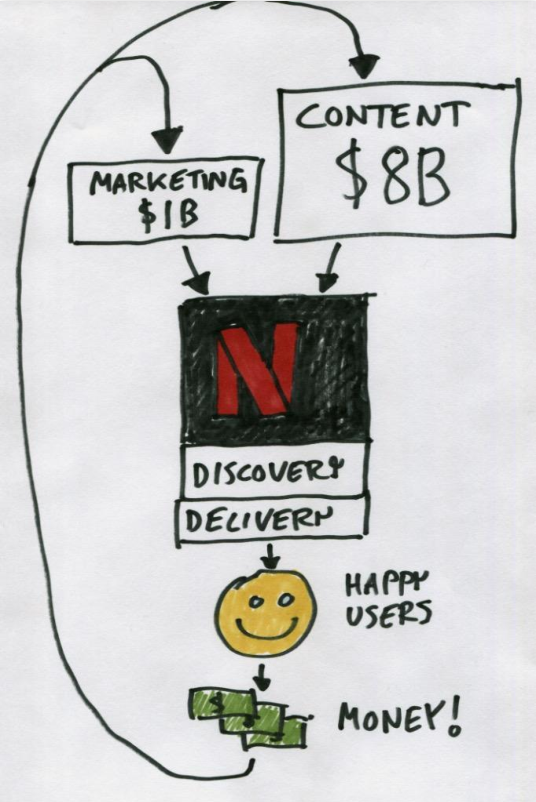
\includegraphics[width=0.5\textwidth,height=\textheight]{img/netflix1.png}

}

\end{figure}

\endcol
\endcols
\end{frame}

\begin{frame}{Machine Learning examples\footnote{Savin Goyal - useR'19}}
\protect\hypertarget{machine-learning-examples-2}{}
\begincols
\begincol{.4\textwidth}

It is probably necessary to \textbf{get smarter} about everything:

\begin{itemize}
\tightlist
\item
  Content acquisition
\item
  Marketing
\item
  Discovery
\item
  Delivery
\item
  and more.
\end{itemize}

ML gets applied everywhere! \endcol

\begincol{.6\textwidth}

\begin{figure}

{\centering 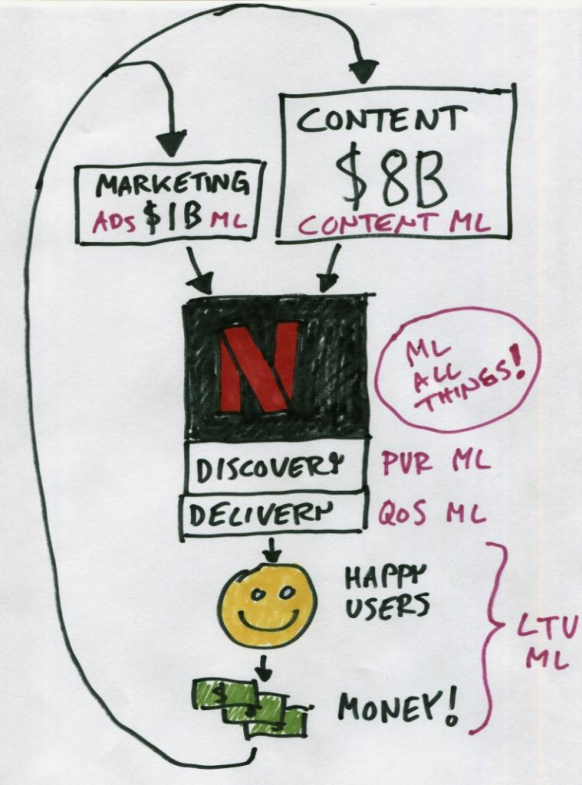
\includegraphics[width=0.6\textwidth,height=\textheight]{img/netflix2.png}

}

\end{figure}

\endcol
\endcols
\end{frame}

\begin{frame}{Machine Learning examples\footnote{Savin Goyal - useR'19}}
\protect\hypertarget{machine-learning-examples-3}{}
\begin{figure}

{\centering 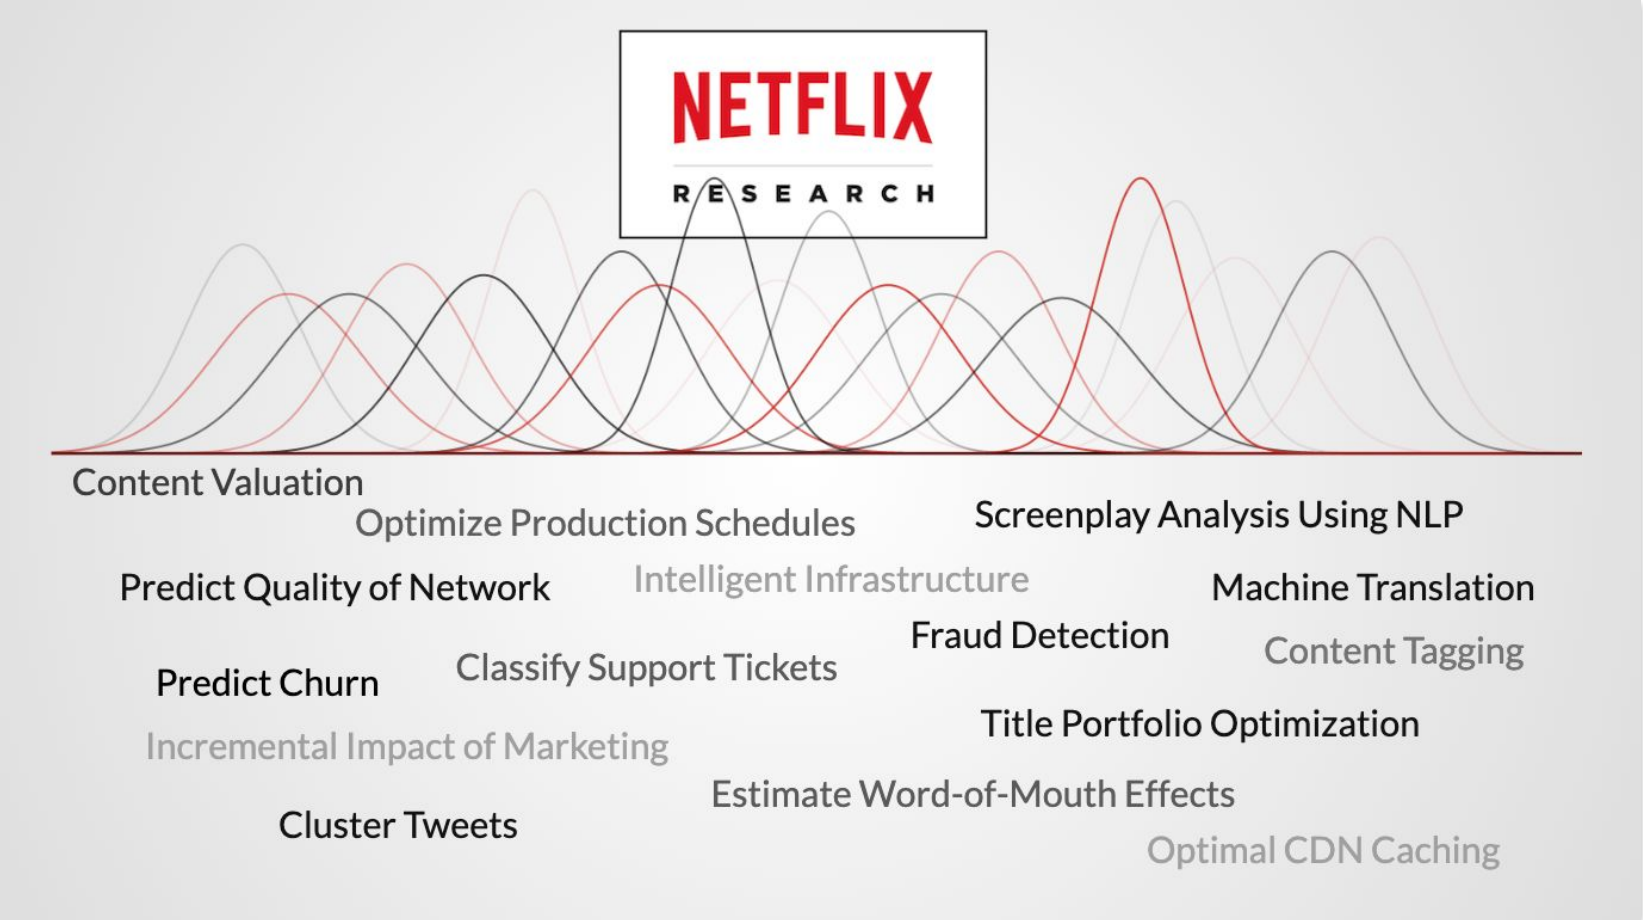
\includegraphics[width=0.8\textwidth,height=\textheight]{img/netflix3.png}

}

\end{figure}
\end{frame}

\begin{frame}{ML is everywhere}
\protect\hypertarget{ml-is-everywhere}{}

\includegraphics[width=0.3\textwidth,height=\textheight]{img/Screenshot_20211118-215613_Twitter.jpg}
\end{frame}

\begin{frame}{Machine Learning: Definition}
\protect\hypertarget{machine-learning-definition}{}
\begin{block}{What is Machine Learning?}
  \begin{itemize}
    \item A science of getting computers to learn without being explicitly programmed\footnote{Arthur Samuel.}.
    % \item A more modern definition: ``A computer program is said to \textcolor{barcolor}{learn from experience E} with respect to \alert{some class of tasks T} and \alert{performance measure P}, if \textcolor{blue}{its performance at tasks in T, as measured by P, improves with experience E}''.
    \item Study of algorithms that \alert{improve} their \textcolor{blue}{performance P} at \textcolor{blue}{some task T} with \textcolor{blue}{experience E}\footnote{Tom Mitchell.}.
  \end{itemize}
\end{block}

\begin{figure}

{\centering 
\includegraphics[width=0.6\textwidth,height=\textheight]{img/ocr.pdf}

}

\end{figure}

\begin{itemize}
  \item[\textcolor{barcolor}{T:}] recognition of a handwritten letter ``a'' from its image.
  \item[\textcolor{barcolor}{E:}] images of a handwritten ``a''.
  \item[\textcolor{barcolor}{P:}] recognition rate.
\end{itemize}
\end{frame}

\begin{frame}{Types of Machine Learning Problems}
\protect\hypertarget{types-of-machine-learning-problems}{}
In general, any machine learning problem can be assigned to one of two
broad types:

\begin{figure}

{\centering \includegraphics[width=0.4\textwidth,height=\textheight]{img/Capture d’écran 2022-07-06 à 17.15.11.png}

}

\end{figure}
\end{frame}

\hypertarget{supervised-learning}{%
\section{Supervised Learning}\label{supervised-learning}}

\begin{frame}{Example: House price
prediction\footnote{Examples from Andrew Ng's MOOC.}}
\protect\hypertarget{example-house-price-prediction}{}
Let's say we want to predict housing prices. We plot a data set and it
looks like this:

\begin{center}
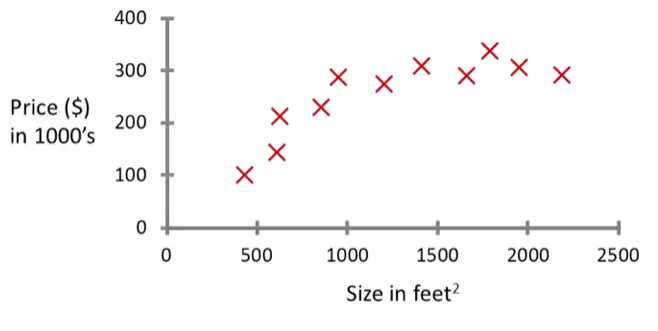
\includegraphics[width=250px]{img/sl1} 
\end{center}

Let's say we own a house that is, say 750 square feet and hoping to sell
the house and we want to know how much we can get for the house.
\end{frame}

\begin{frame}{Example: Medical diagnosis}
\protect\hypertarget{example-medical-diagnosis}{}
Let's say a person has a breast tumor, and her breast tumor size is
known.

\begin{center}
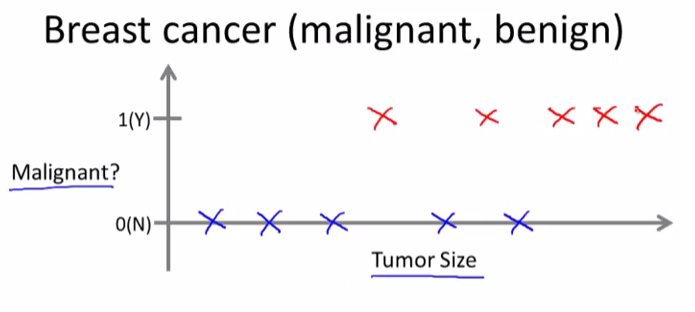
\includegraphics[width=230px]{img/sl5} 
\end{center}
\begin{itemize}
  \item The machine learning question here is, can you estimate what is the \textbf{probability} that a tumor is malignant versus benign?
\end{itemize}
\end{frame}

\begin{frame}{Example: Medical diagnosis}
\protect\hypertarget{example-medical-diagnosis-1}{}
Let's say that we know both the age of the patients and the tumor size.
In that case maybe the data set will look like this.

\begin{center}
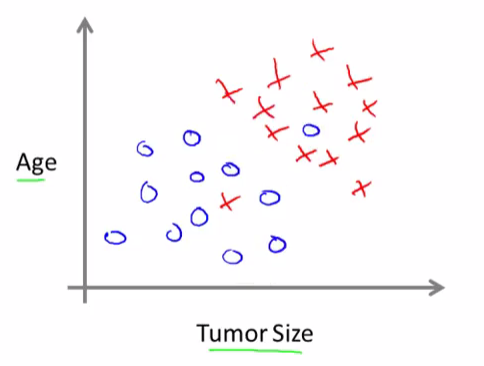
\includegraphics[width=175px]{img/sl9}
\end{center}
\end{frame}

\begin{frame}{Supervised Learning: Definition \& Model}
\protect\hypertarget{supervised-learning-definition-model}{}
The term \textcolor{barcolor}{supervised learning} refers to the fact
that we gave the algorithm a data set in which the
\textbf{``right answers''} (known as \textbf{labels}) were given. \pause

\tikzset{
  basic/.style  = {text width=2.5cm, rectangle,fill=backgroundcolor,draw=barcolor},
  root/.style   = {basic, text width=3.5cm,minimum height=1cm,rounded corners=2pt, thin, align=center},
  level 2/.style = {basic,  text width=3.5cm, rounded corners=2pt, thin, align=center,minimum height=1cm,sibling distance=40mm},
  level 3/.style = {basic,  text width=1.5cm, rounded corners=2pt, thin, text=black,align=center,minimum height=1cm,sibling distance=40mm}
                  }

\begin{center}
\begin{tikzpicture}[level 1/.style={sibling distance=70mm},
  edge from parent/.style={->,draw,barcolor},
  >=latex]

% root of the the initial tree, level 1
\node[root] {\large{Training Set}}
% The first level, as children of the initial tree
    child { node[level 2] (n) {\large{Learning Algorithm}} 
     child { node[level 3] (f) {\Huge $f$} }
     }
;

\node (target) [right of=f, xshift=1.6cm] {\Large Target};

\node (features) [left of=f, xshift=-1.6cm] {\Large Features};

\tikzstyle{arrow} = [->,draw,barcolor]

\draw [arrow] (f) -- (target);
\draw [arrow] (features) -- (f);

\end{tikzpicture}
\end{center}

\begin{itemize}
\tightlist
\item Supervised Learning refers to a set of approaches for
  \textcolor{blue}{estimating $f$}.
\item \(f\) is also called \textbf{\emph{\textcolor{red}{hypothesis}}} in
  Machine Learning.
\end{itemize}
\end{frame}

\begin{frame}{Regression vs Classification}
\protect\hypertarget{regression-vs-classification}{}
\begincols
\begincol{.45\textwidth}
\begin{block}{Regression}
\begin{itemize}
\item The example of the house price prediction is also called a
  \alert{regression} problem.
\item A regression problem is when we try to predict a \alert{quantitative
  (continuous)} value output. Namely the price in the example.
\end{itemize}
\end{block}

\endcol

\begincol{.45\textwidth}
\begin{block}{Classification}
\begin{itemize}
\item The process for predicting \alert{qualitative (categorical,
  discrete)} responses is known as classification.
\item Methods: Logistic regression, Support Vector Machines, etc..
\end{itemize}
\end{block}

\endcol
\endcols
\end{frame}

\begin{frame}{Supervised Learning: Notations}
\protect\hypertarget{supervised-learning-notations}{}
Notations:

\begin{itemize}
\item The size of the house in the first example, tumor size and age in the second example, are the \textbf{\textcolor{barcolor}{input}} variables. Typically
  denoted by \(X\).
\item The inputs go by different names, such as
  \emph{\textcolor{blue}{predictors}},
  \emph{\textcolor{blue}{independent variables}},
  \emph{\textcolor{blue}{features}}, \emph{\textcolor{blue}{predictor}}
  or sometimes just \emph{\textcolor{blue}{variables}}.  \pause
\item The house price in the first example and the diagnosis in the second example are the \textbf{\textcolor{barcolor}{output}} variables, and are typically
  denoted using the symbol \(Y\).
\item The output variable is often called the
  \emph{\textcolor{red}{response}},
  \emph{\textcolor{red}{dependent variable}} or
  \emph{\textcolor{red}{target}}.
\end{itemize}
\end{frame}

\hypertarget{unsupervised-learning}{%
\section{Unsupervised Learning}\label{unsupervised-learning}}

\begin{frame}{Unsupervised Learning: ``No labels'\,'}
\protect\hypertarget{unsupervised-learning-no-labels}{}
In Unsupervised Learning, we're given data that doesn't have any
\textbf{labels}.

For example:

\begin{center}
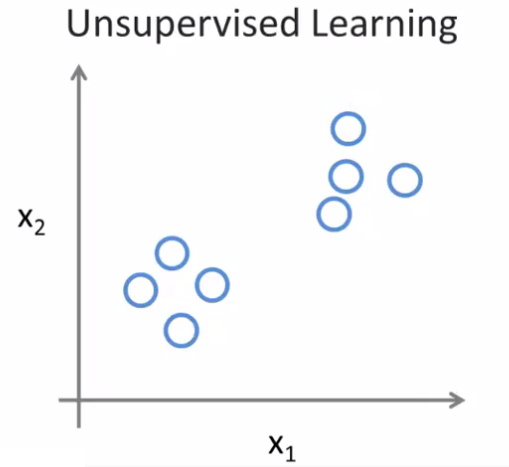
\includegraphics[width=150px]{img/ul1}
\end{center}

Question: Can you find some structure in the data?
\end{frame}

\begin{frame}{Unsupervised Learning: Example}
\protect\hypertarget{unsupervised-learning-example}{}
One example where clustering is used is in Google News (news.google.com)

\begin{center}
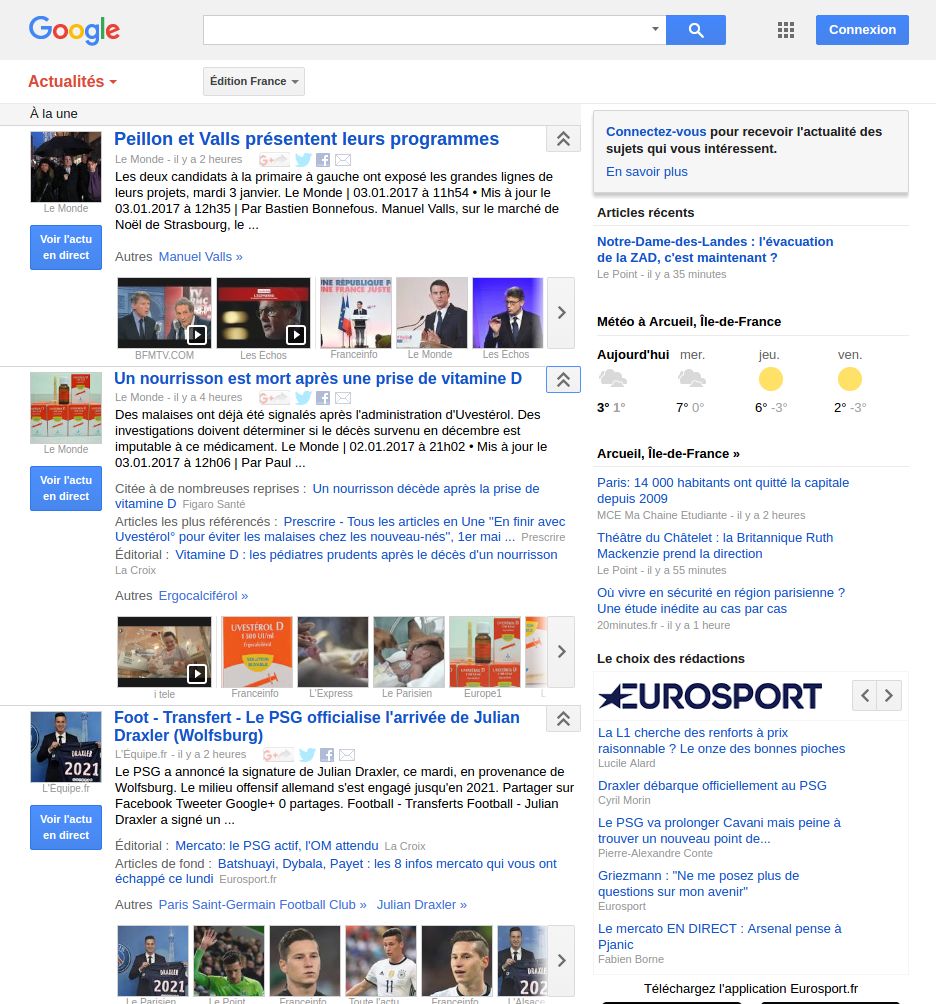
\includegraphics[width=180px]{img/googlenews}
\end{center}
\end{frame}

\begin{frame}{Types of Machine Learning Problems}
\protect\hypertarget{types-of-machine-learning-problems-1}{}
\tikzset{
  % basic/.style  = {text width=2.5cm, text=white, rectangle},
  basic/.style  = {text width=2.5cm, fill=white,draw=barcolor, rectangle},
  root/.style   = {basic, minimum height=0.7cm, text width=3.5cm,rounded corners=2pt, thin, align=center},
  level 2/.style = {basic, minimum height=0.7cm, text width=3.5cm, rounded corners=2pt, thin, align=center,sibling distance=40mm,draw=barcolor!80},
 level 3/.style = {basic, rounded corners=2pt, thin, align=center,font=\small,draw=barcolor!60},
level 33/.style = {basic, text width=2.5cm,rounded corners=2pt, thin, align=center,
                   fill=white, draw=barcolor,font=\small,draw=barcolor!60},
  level 4/.style = {basic, rounded corners=2pt, thin, align=center,draw=barcolor!40},
    level 5/.style = {basic, rounded corners=2pt, thin, align=center,font=\small,draw=barcolor!20}
}

\begin{center}
\begin{tikzpicture}[scale=0.8,
  level 1/.style={sibling distance=70mm},
  edge from parent/.style={->,draw,barcolor},
  >=latex]

% root of the the initial tree, level 1
\node[root] {Machine Learning Types}
% The first level, as children of the initial tree
    child { node[level 2] {Supervised Learning} 
          child { node[level 3] {Continuous Target Variable}
            child { node[level 4] {Regression}
              child { node[level 5] {House Price \\ Prediction}}}}
          child { node[level 3] {Categorical Target Variable}
            child { node[level 4] {Classification}
              child { node[level 5] {Medical diagnosis}}}}
      }
    child { node[level 2] {Unsupervised Learning}
      child { node[level 33] {Target Variable Not Available}
        child { node[level 4] {Clustering}
          child { node[level 5] {Customer segmentation}}}
         } 
    }
;
\end{tikzpicture}
\end{center}
\end{frame}

\hypertarget{linear-regression}{%
\section{Linear Regression}\label{linear-regression}}

\begin{frame}{Regression}
\protect\hypertarget{regression}{}
\begincols

\begincol{.6\textwidth}

\begin{figure}

{\centering 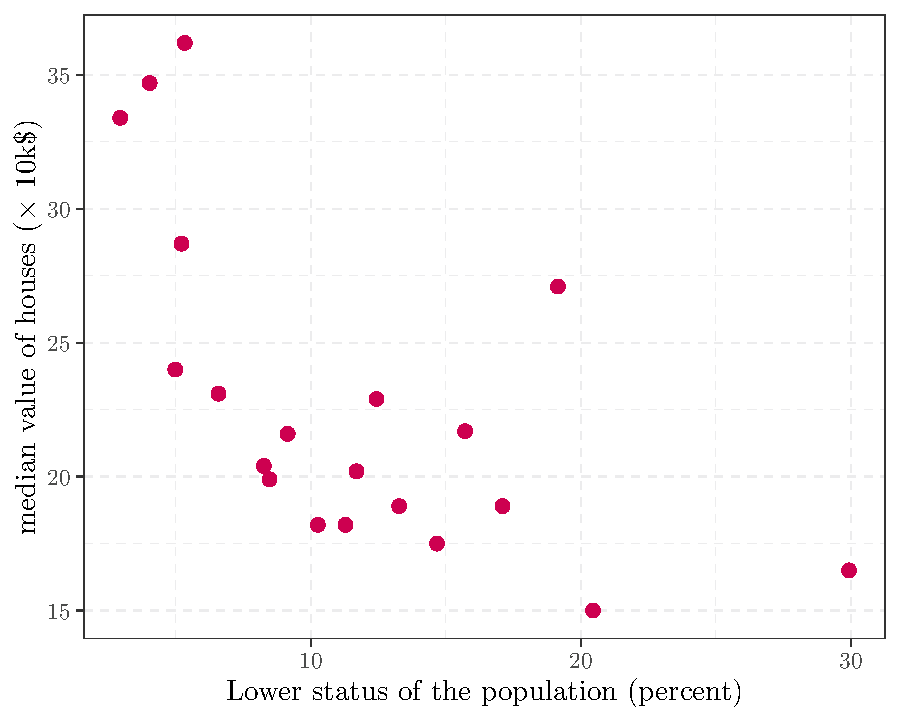
\includegraphics[width=0.5\textwidth,height=\textheight]{CM1_Machine_Learning_files/figure-beamer/unnamed-chunk-7-1.pdf}

}

\end{figure}

\endcol
\begincol{.4\textwidth}

Let:

\begin{itemize}
\tightlist
\item
  \(n\): sample size
\item
  \(x\): features
\item
  \(y\): target variable
\item
  \((x^{(i)},y^{(i)})\): one sample, a training example
\end{itemize}

\endcol
\endcols
\end{frame}

\begin{frame}{Simple Linear Regression}
\protect\hypertarget{simple-linear-regression}{}
\begincols
\begincol{.4\textwidth}

\begin{figure}

{\centering 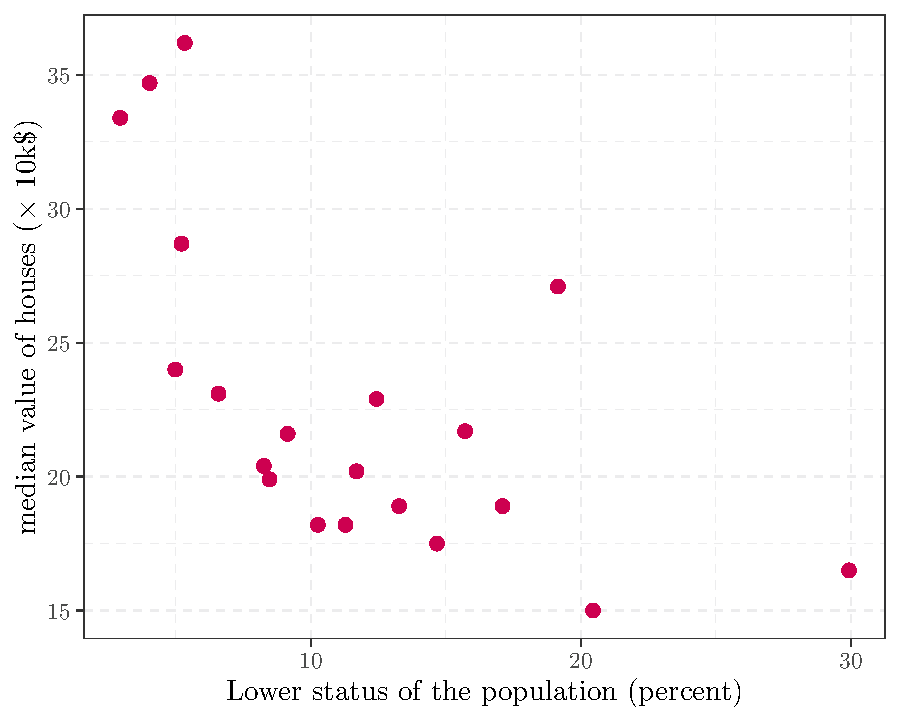
\includegraphics[width=0.7\textwidth,height=\textheight]{CM1_Machine_Learning_files/figure-beamer/unnamed-chunk-8-1.pdf}

}

\end{figure}

\endcol

\begincol{.6\textwidth}

\begin{itemize}
\tightlist
\item
  Hypothesis: \(f(x) = f_{\omega}(x) = \omega_0 + \omega_1 x\)
\item
  Choose \(\omega_0\) and \(\omega_1\) so that \(f_{\omega}(x)\) is
  close to \(y\)
\item
  \alert{Cost function} \(J(\omega) =\)
\item
  How to calculate \(\omega\)?

  \begin{itemize}
  \tightlist
  \item
    GD
  \item
    OLS
  \end{itemize}
\end{itemize}

\endcol
\endcols
\end{frame}

\begin{frame}{Cost function intuition}
\protect\hypertarget{cost-function-intuition}{}
\begin{block}{Simple linear regression}

\begin{itemize}
\tightlist
\item
  Model: \(f_{\omega}(x) = \omega_0 + \omega_1 x = \omega'x\)
\item
  Parameters: \(\omega_0\) and \(\omega_1\)
\item
  Cost function:
  \(J(\omega_0,\omega_1) = \frac{1}{2 n} \sum_{i=1}^{n}\left(f_{\omega}\left(x^{(i)}\right)-y^{(i)}\right)^{2}\)
\item
  Goal: \(\min_{\omega_0,\omega_1} J(\omega_0,\omega_1)\)
\end{itemize}

\end{block}

\vspace{1cm}

Suppose a \alert{simplified} hypothesis (with 1 parameter):

\begin{itemize}
\tightlist
\item
  Model: Let \(f_{\omega}(x) = \omega_1 x = \omega'x\)
\item
  Parameter: \(\omega_1\)
\item
  Cost function:
  \(J(\omega_1) = \frac{1}{2 n} \sum_{i=1}^{n}\left(f_{\omega}\left(x^{(i)}\right)-y^{(i)}\right)^{2}\)
\end{itemize}
\end{frame}

\begin{frame}{Cost function intuition}
\protect\hypertarget{cost-function-intuition-1}{}
\begincols
\begincol{.5\textwidth}

Let the following example:

\begin{figure}

{\centering 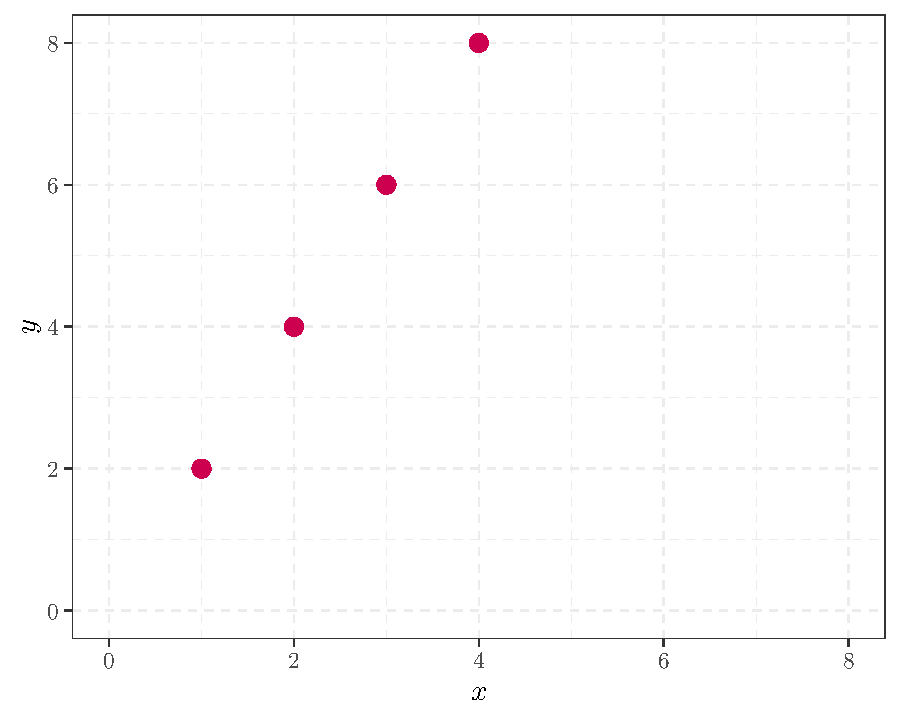
\includegraphics[width=0.6\textwidth,height=\textheight]{CM1_Machine_Learning_files/figure-beamer/unnamed-chunk-9-1.pdf}

}

\end{figure}

\endcol
\begincol{.5\textwidth}

\begin{figure}

{\centering 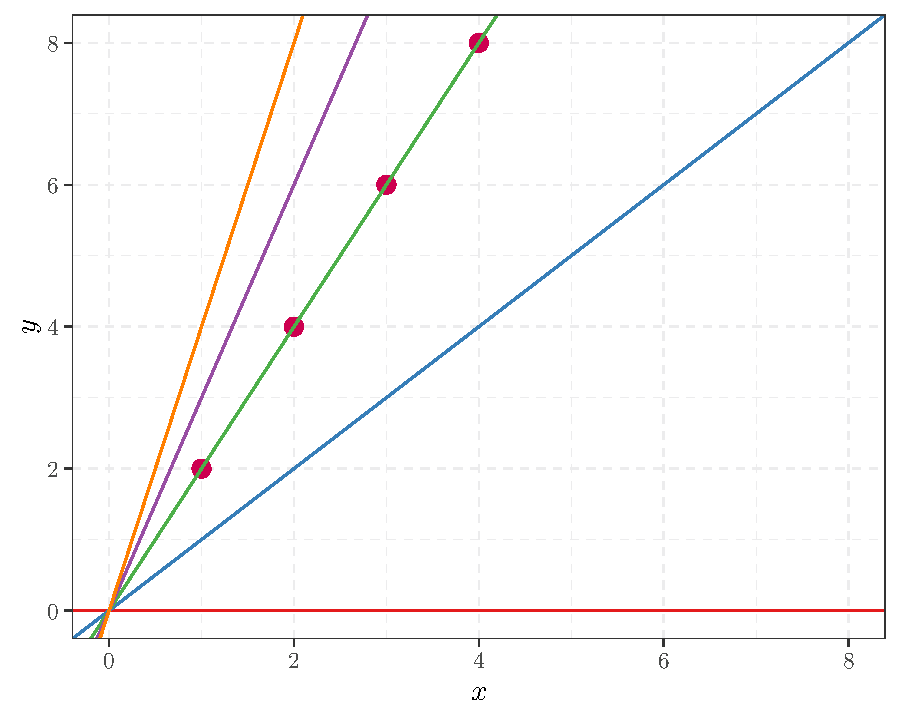
\includegraphics[width=0.6\textwidth,height=\textheight]{CM1_Machine_Learning_files/figure-beamer/unnamed-chunk-10-1.pdf}

}

\end{figure}

\begin{figure}

{\centering 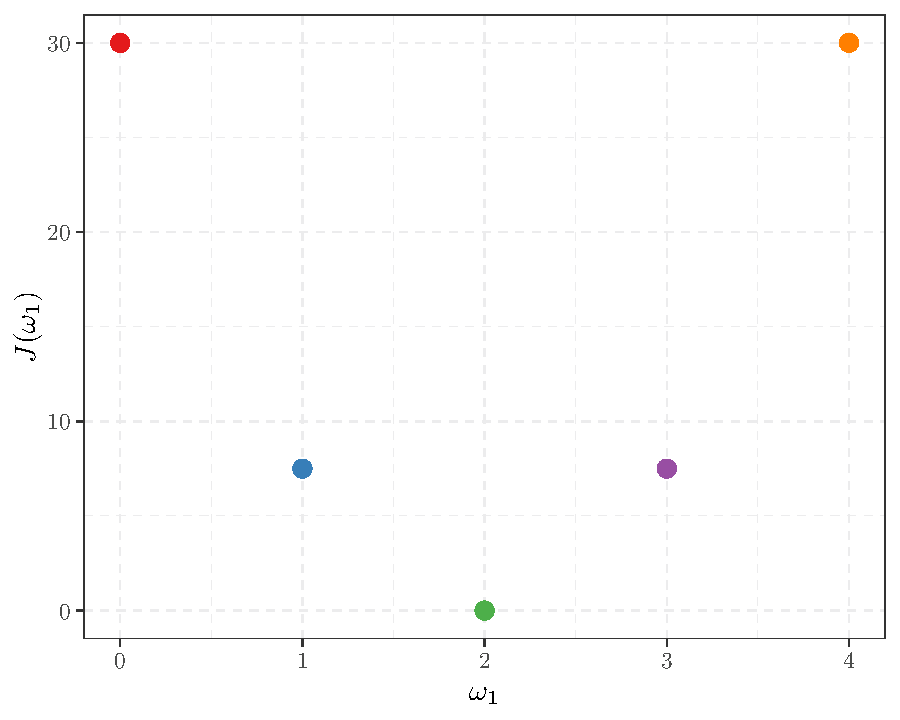
\includegraphics[width=0.6\textwidth,height=\textheight]{CM1_Machine_Learning_files/figure-beamer/unnamed-chunk-10-2.pdf}

}

\end{figure}

\endcol
\endcols
\end{frame}

\begin{frame}{Cost function intuition}
\protect\hypertarget{cost-function-intuition-2}{}
\begin{block}{Simple linear regression}

\begin{itemize}
\tightlist
\item
  Model: \(f_{\omega}(x) = \omega_0 + \omega_1 x = \omega'x\)
\item
  Cost function:
  \(J(\omega_0,\omega_1) = \frac{1}{2 n} \sum_{i=1}^{n}\left(f_{\omega}\left(x^{(i)}\right)-y^{(i)}\right)^{2}\)
\end{itemize}

\end{block}

\begin{figure}

\begin{minipage}[t]{0.33\linewidth}

{\centering 

\raisebox{-\height}{

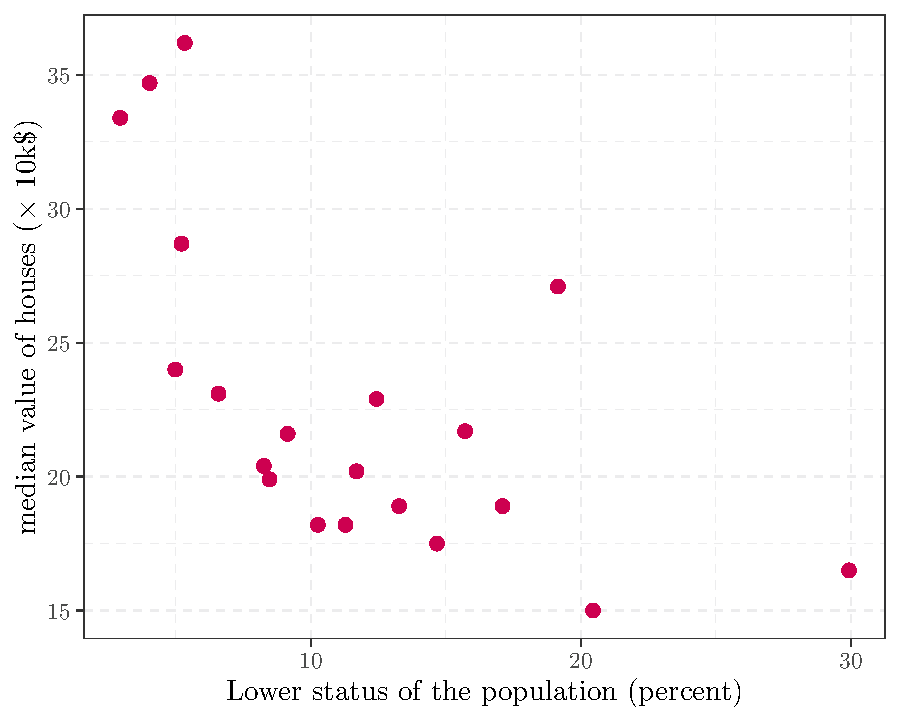
\includegraphics[width=1.7in,height=\textheight]{CM1_Machine_Learning_files/figure-beamer/unnamed-chunk-11-1.pdf}

}

}

\end{minipage}%
%
\begin{minipage}[t]{0.33\linewidth}

{\centering 

\raisebox{-\height}{

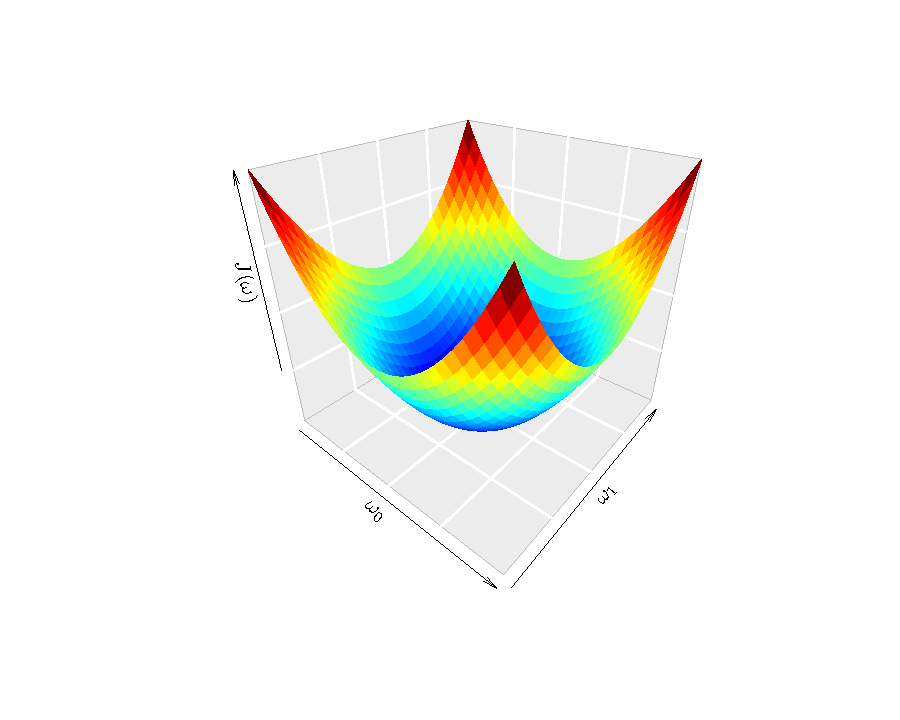
\includegraphics[width=1.7in,height=\textheight]{CM1_Machine_Learning_files/figure-beamer/unnamed-chunk-11-2.pdf}

}

}

\end{minipage}%
%
\begin{minipage}[t]{0.33\linewidth}

{\centering 

\raisebox{-\height}{

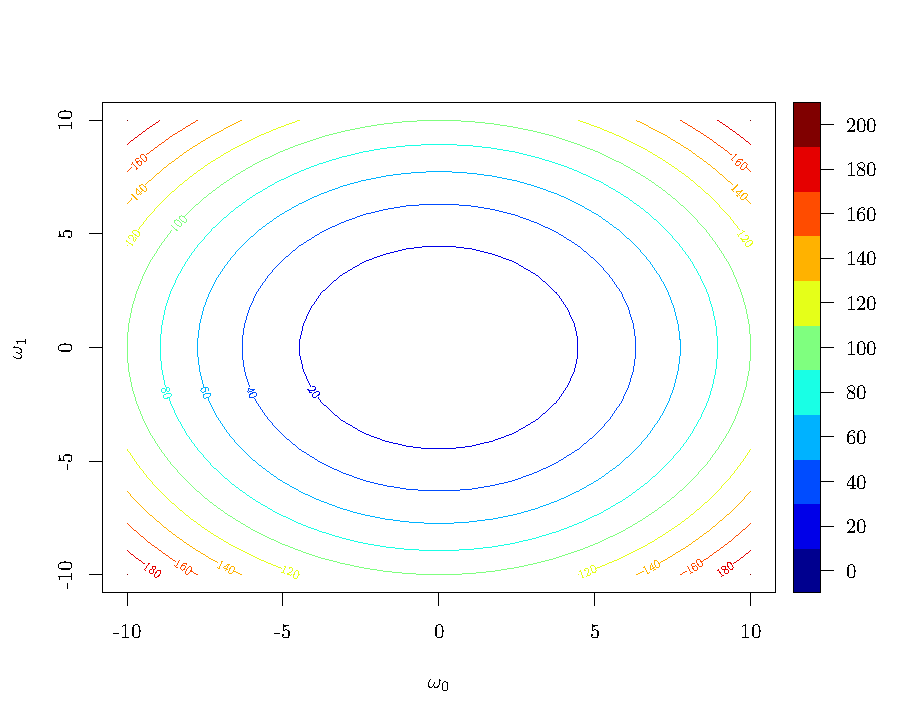
\includegraphics[width=1.7in,height=\textheight]{CM1_Machine_Learning_files/figure-beamer/unnamed-chunk-11-3.pdf}

}

}

\end{minipage}%

\end{figure}
\end{frame}

\begin{frame}{Multiple Linear Regression}
\protect\hypertarget{multiple-linear-regression}{}
\begincols

\begincol{.7\textwidth}

\begin{itemize}
\tightlist
\item
  Let \(p\) features: \(x_1, x_2, \ldots, x_p\)
\item
  Multiple linear regression:
  \(f(x) = f_{\omega}(x) = \omega_0 + \omega_1 x_1 + \ldots + \omega_p x_p\)
\end{itemize}

\begin{figure}

{\centering 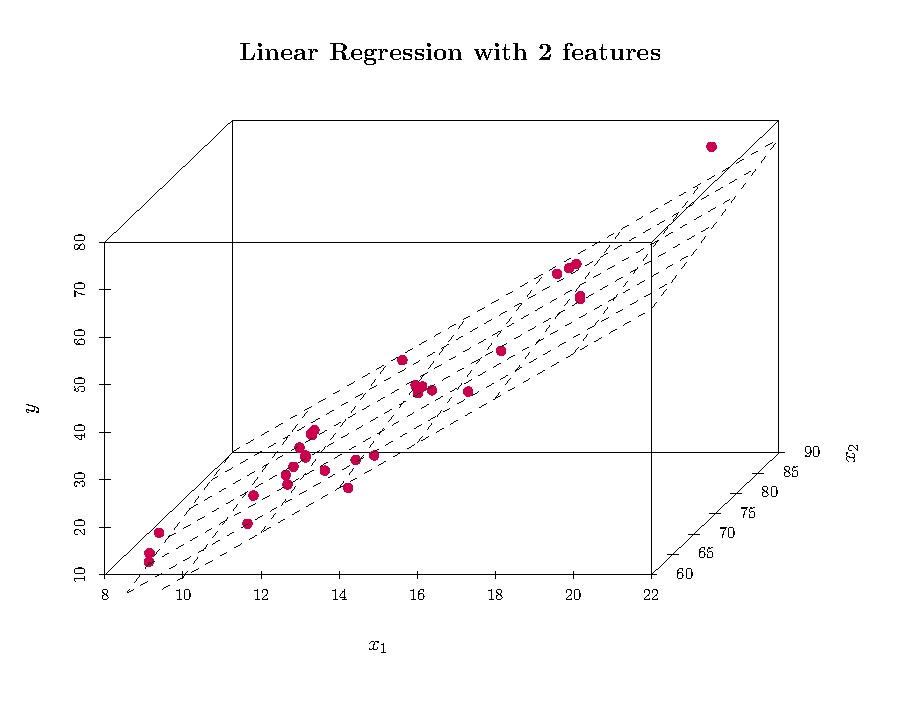
\includegraphics[width=0.7\textwidth,height=\textheight]{CM1_Machine_Learning_files/figure-beamer/unnamed-chunk-12-1.pdf}

}

\end{figure}

\endcol
\begincol{.3\textwidth}
\endcol
\endcols
\end{frame}

\begin{frame}{Multiple Linear Regression}
\protect\hypertarget{multiple-linear-regression-1}{}
\begincols

\begincol{.7\textwidth}

\begin{itemize}
\tightlist
\item
  Let \(p\) variables: \(x_1, x_2, \ldots, x_p\)
\item
  Multiple linear regression:
  \(f(x) = f_{\omega}(x) = \omega_0 + \omega_1 x_1 + \ldots + \omega_p x_p\)
\item
  Define \(x_0 = 1\), and
\end{itemize}

\[\omega = \begin{pmatrix}
    \omega_{0} \\
    \omega_{1} \\
    \vdots \\
    \omega_{p}
    \end{pmatrix}    \quad  x = \begin{pmatrix}
    x_{0} \\
    x_{1} \\
    \vdots \\
    x_{p}
    \end{pmatrix}\]

\begin{itemize}
\tightlist
\item
  Using matrices: \(f_{\omega}(x) = \omega' x\)
\item
  Methods to estimate \(\omega\):

  \begin{itemize}
  \tightlist
  \item
    OLS
  \item
    GD
  \end{itemize}
\item
  Cost function
  \(J(\omega) = \frac{1}{2 n} \sum_{i=1}^{n}\left(f_{\omega}\left(x^{(i)}\right)-y^{(i)}\right)^{2}\)
\end{itemize}

\endcol
\begincol{.3\textwidth}
\endcol
\endcols
\end{frame}

\hypertarget{gradient-descent}{%
\section{Gradient descent}\label{gradient-descent}}

\begin{frame}[fragile]{Gradient descent: algorithm}
\protect\hypertarget{gradient-descent-algorithm}{}
\begincols

\begincol{.7\textwidth}

\begin{itemize}
\item
  Let a function \(J(\theta)\)
\item
  \textbf{Goal}: Find \(\theta\) that minimizes \(J(\theta)\),
  e.g.~\(\theta = \argmin_{\theta} J(\theta)\)
\item
  \textbf{Algorithm}:

  \begin{itemize}
  \tightlist
  \item
    \texttt{initialize} \(\theta\) \texttt{randomly}
  \item
    \texttt{repeat\ until\ convergence}\{
  \end{itemize}
\end{itemize}

\[\theta^{new} = \theta^{old} - \alpha J'(\theta)\]

\text{                            } \}

\begin{itemize}
\tightlist
\item
  \(\alpha\) is the learning rate
\end{itemize}

\endcol
\begincol{.3\textwidth}
\endcol
\endcols
\end{frame}

\begin{frame}{Gradient descent: convex functions}
\protect\hypertarget{gradient-descent-convex-functions}{}
\begin{exampleblock}{Convex function}

\begin{itemize}
\tightlist
\item
  \(f\) is convex if
  \(f\left(\lambda x_{1}+(1-\lambda) x_{2}\right) \leq \lambda f\left(x_{1}\right)+(1-\lambda) f\left(x_{2}\right), \forall x_{1}\)
  and \(x_{2} \in d_f, \lambda \in(0,1)\).
\item
  \(f\) is convex iff \(f'' \geq 0\)
\item
  A convex funtion has a global minimum
\end{itemize}

\end{exampleblock}

\begin{figure}

\begin{minipage}[t]{0.50\linewidth}

{\centering 

\raisebox{-\height}{

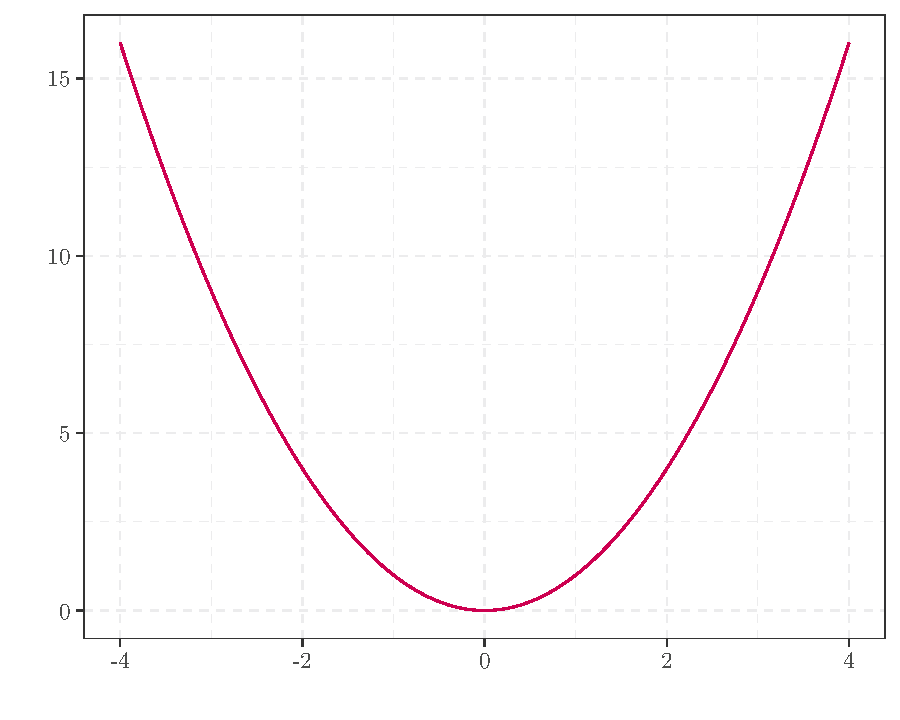
\includegraphics[width=2in,height=\textheight]{CM1_Machine_Learning_files/figure-beamer/unnamed-chunk-13-1.pdf}

}

}

\end{minipage}%
%
\begin{minipage}[t]{0.50\linewidth}

{\centering 

\raisebox{-\height}{

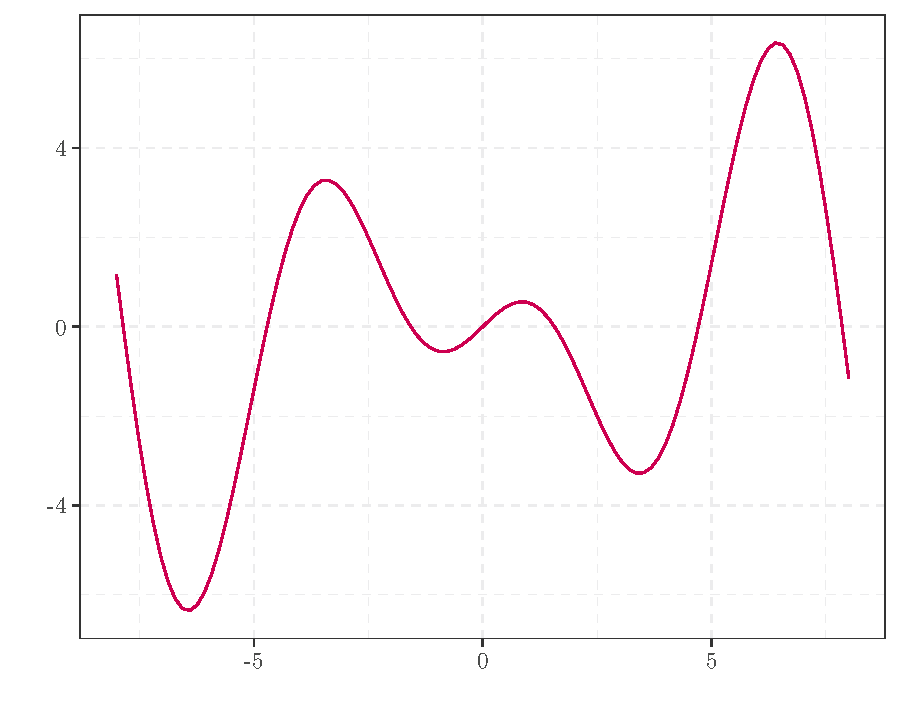
\includegraphics[width=2in,height=\textheight]{CM1_Machine_Learning_files/figure-beamer/unnamed-chunk-13-2.pdf}

}

}

\end{minipage}%

\end{figure}
\end{frame}

\begin{frame}{Gradient descent: example}
\protect\hypertarget{gradient-descent-example}{}
\begincols
\begincol{.2\textwidth}

\begin{itemize}
\tightlist
\item
  Let \(J(\theta)=\theta^2\)
\item
  So \(J'(\theta) = 2 \theta\)
\item
  Let \(\alpha = 0.1\)
\end{itemize}

\endcol

\begincol{.8\textwidth}

\begin{figure}

{\centering 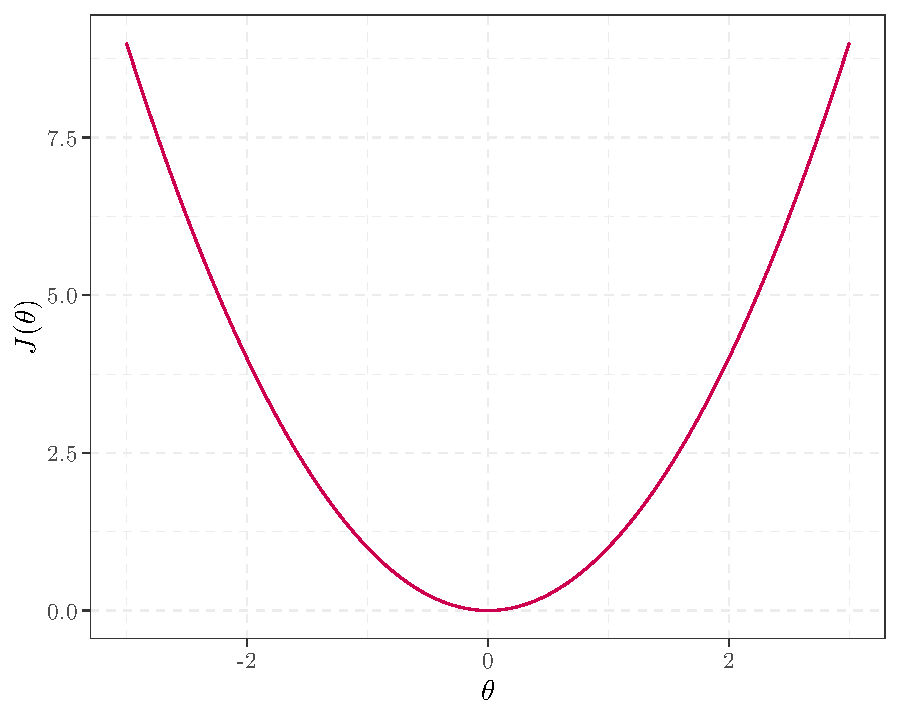
\includegraphics[width=0.5\textwidth,height=\textheight]{CM1_Machine_Learning_files/figure-beamer/unnamed-chunk-14-1.pdf}

}

\end{figure}

\endcol
\endcols
\end{frame}

\begin{frame}{Gradient descent: choosing \(\alpha\)}
\protect\hypertarget{gradient-descent-choosing-alpha}{}
\begin{itemize}
\tightlist
\item
  \(J(\theta)\) must decrease after each iteration
\item
  Define the convergence
\end{itemize}

\begin{figure}

\begin{minipage}[t]{0.50\linewidth}

{\centering 

\raisebox{-\height}{

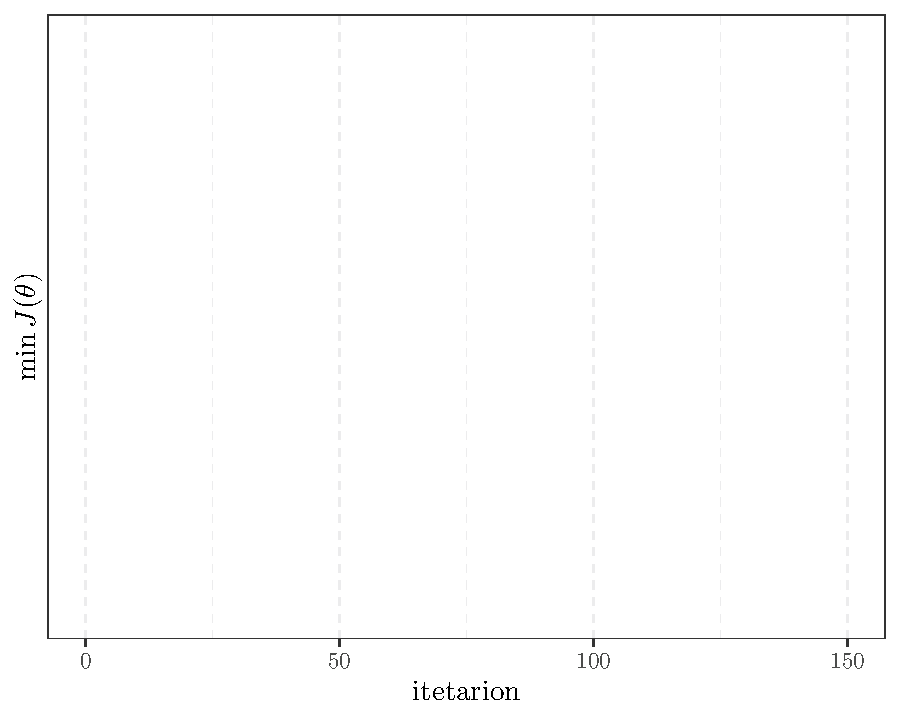
\includegraphics[width=2in,height=\textheight]{CM1_Machine_Learning_files/figure-beamer/unnamed-chunk-15-1.pdf}

}

}

\end{minipage}%
%
\begin{minipage}[t]{0.50\linewidth}

{\centering 

\raisebox{-\height}{

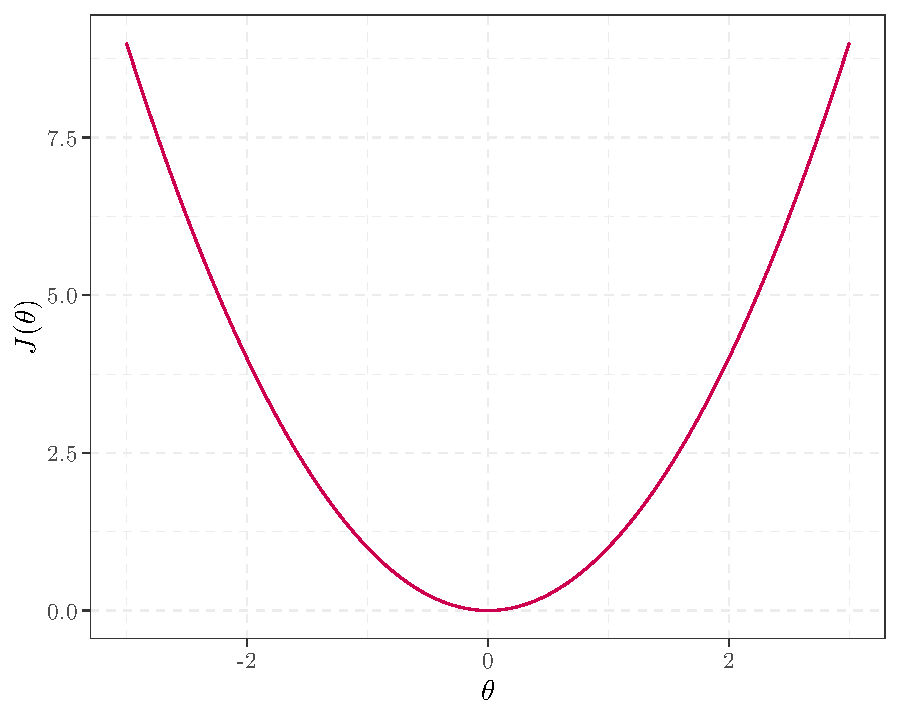
\includegraphics[width=2in,height=\textheight]{CM1_Machine_Learning_files/figure-beamer/unnamed-chunk-15-2.pdf}

}

}

\end{minipage}%

\end{figure}

\begin{itemize}
\tightlist
\item
  If \(\alpha\) is too small, slow convergence
\item
  If \(\alpha\) is too large, convergence is not guaranteed
\end{itemize}
\end{frame}

\begin{frame}[fragile]{Gradient descent: function of two variables}
\protect\hypertarget{gradient-descent-function-of-two-variables}{}
\begin{itemize}
\item
  Let a function \(J(\theta_0, \theta_1)\)
\item
  \textbf{Goal}: find \((\theta_0,\theta_1)\) that minimize
  \(J(\theta_0, \theta_1)\),
  e.g.~\(\argmin_{(\theta_0,\theta_1)} J(\theta_0, \theta_1)\)
\item
  \textbf{Algorithm}:

  \begin{itemize}
  \tightlist
  \item
    \texttt{initialize} \((\theta_0,\theta_1)\) \texttt{randomly}
  \item
    \texttt{repeat\ until\ convergence}\{
  \end{itemize}
\end{itemize}

\[\theta_0^{new} = \theta_0^{old} - \alpha \frac{\partial }{\partial \theta_0} J(\theta_0, \theta_1)\]

\[\theta_1^{new} = \theta_1^{old} - \alpha \frac{\partial }{\partial \theta_1} J(\theta_0, \theta_1)\]

\text{                            } \}

\begin{itemize}
\tightlist
\item
  \(\alpha\) is the learning rate
\item
  Same principle if \(J\) is a function of more variables
\end{itemize}
\end{frame}

\begin{frame}{Gradient descent: function of two variables}
\protect\hypertarget{gradient-descent-function-of-two-variables-1}{}
\begin{figure}

\begin{minipage}[t]{0.33\linewidth}

{\centering 

\raisebox{-\height}{

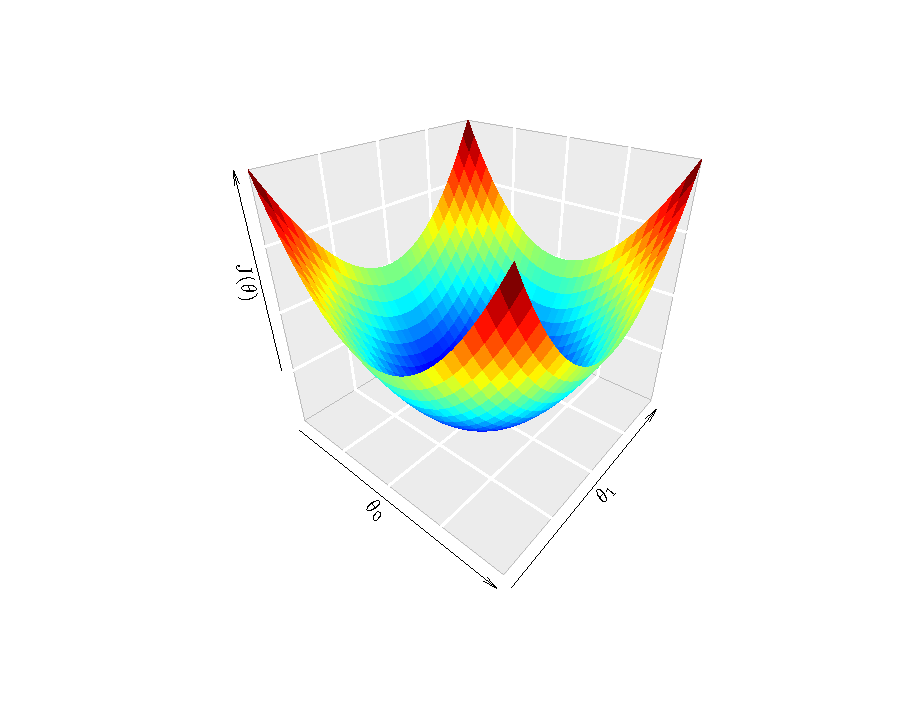
\includegraphics[width=1.7in,height=\textheight]{CM1_Machine_Learning_files/figure-beamer/unnamed-chunk-16-1.pdf}

}

}

\end{minipage}%
%
\begin{minipage}[t]{0.33\linewidth}

{\centering 

\raisebox{-\height}{

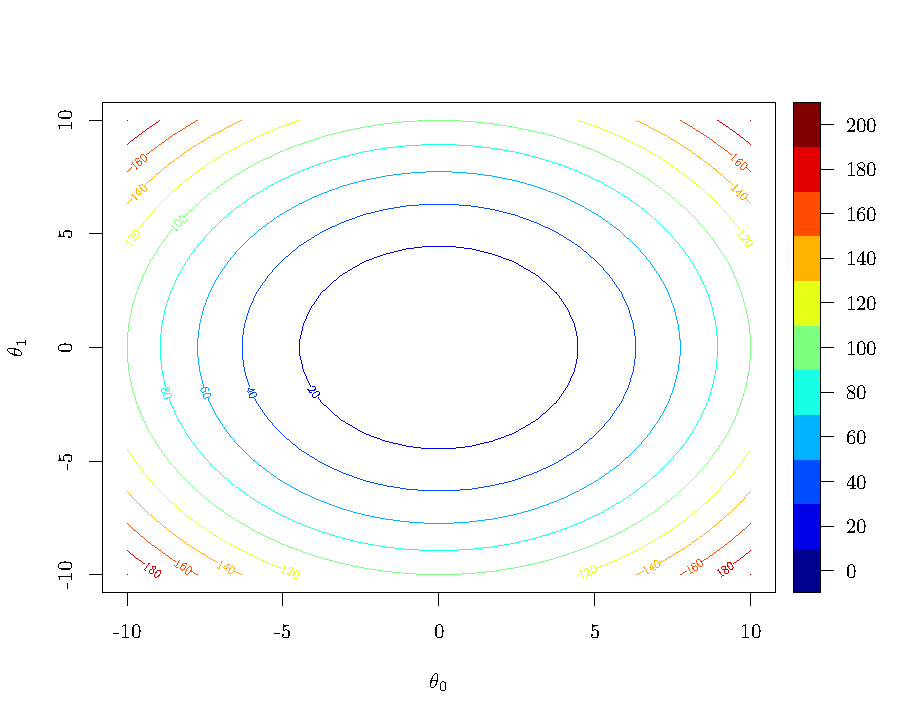
\includegraphics[width=1.7in,height=\textheight]{CM1_Machine_Learning_files/figure-beamer/unnamed-chunk-16-2.pdf}

}

}

\end{minipage}%
%
\begin{minipage}[t]{0.33\linewidth}

{\centering 

\raisebox{-\height}{

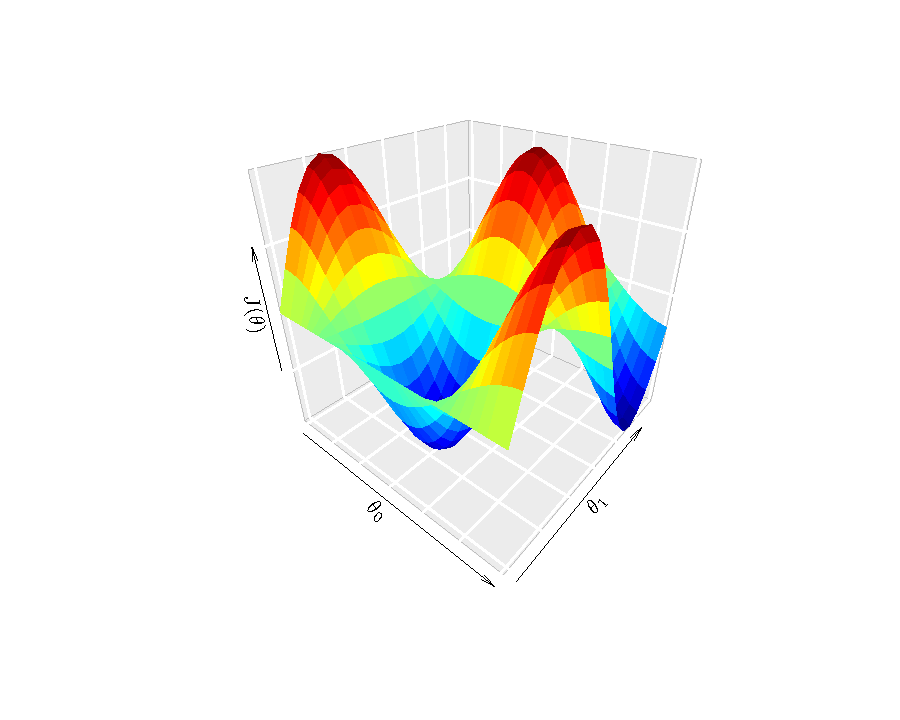
\includegraphics[width=1.7in,height=\textheight]{CM1_Machine_Learning_files/figure-beamer/unnamed-chunk-16-3.pdf}

}

}

\end{minipage}%

\end{figure}
\end{frame}

\begin{frame}[fragile]{Gradient descent for linear regression}
\protect\hypertarget{gradient-descent-for-linear-regression}{}
\begin{block}{Simple linear regression}

\begin{itemize}
\tightlist
\item
  Model: \(f_{\omega}(x) = \omega_0 + \omega_1 x = \omega'x\)
\item
  Parameters: \(\omega_0\) and \(\omega_1\)
\item
  Cost function:
  \(J(\omega_0,\omega_1) = \frac{1}{2 n} \sum_{i=1}^{n}\left(f_{\omega}\left(x^{(i)}\right)-y^{(i)}\right)^{2}\)
\item
  Goal: \(\min_{\omega_0,\omega_1} J(\omega_0,\omega_1)\)
\end{itemize}

\end{block}

\begincols
\begincol{.49\textwidth}

\begin{alertblock}{Algorithm}

\begin{itemize}
\tightlist
\item
  \texttt{initialize} \((\omega_0,\omega_1)\) \texttt{randomly}
\item
  \texttt{repeat\ until\ convergence}\{
\end{itemize}

\[\omega_i^{new} = \omega_i^{old} - \alpha \frac{\partial }{\partial \omega_i} J(\omega_0, \omega_1)\]

\[\text{for } i = 0 \text{ and } i=1\]

\}

\end{alertblock}

\endcol

\begincol{.49\textwidth}

\begin{alertblock}{Algorithm}

\begin{itemize}
\tightlist
\item
  \texttt{initialize} \((\omega_0,\omega_1)\) \texttt{randomly}
\item
  \texttt{repeat\ until\ convergence}\{ \begin{align*}
  \omega_0^{new} &= \omega_0^{old} - \alpha \frac{1}{n} \sum_{i=1}^{n}\left(f_{\omega}\left(x^{(i)}\right)-y^{(i)}\right) \\
  \omega_1^{new} &= \omega_1^{old} - \alpha \frac{1}{n} \sum_{i=1}^{n}\left(f_{\omega}\left(x^{(i)}\right)-y^{(i)}\right).x^{(i)}
  \end{align*} \}
\end{itemize}

\end{alertblock}

\endcol
\endcols
\end{frame}

\begin{frame}[fragile]{Gradient descent for multiple linear regression}
\protect\hypertarget{gradient-descent-for-multiple-linear-regression}{}
\begin{block}{Multiple linear regression}

\begin{itemize}
\tightlist
\item
  Model:
  \(f_{\omega}(x) = \omega_0 + \omega_1 x_1 + \ldots + \omega_p x_p= \omega'x\)
\item
  Parameters: \(\omega_0, \omega_1, \ldots, \omega_p\)
\item
  Cost function:
  \(J(\omega) = \frac{1}{2 n} \sum_{i=1}^{n}\left(f_{\omega}\left(x^{(i)}\right)-y^{(i)}\right)^{2}\)
\end{itemize}

\end{block}

\begin{alertblock}{Algorithm}

\begin{itemize}
\tightlist
\item
  \texttt{initialize} the \(\omega_i\) \texttt{randomly}
\item
  \texttt{repeat\ until\ convergence}\{
\end{itemize}

\[\omega_i^{new} = \omega_i^{old} - \alpha \frac{\partial }{\partial \omega_i} J(\omega) \quad \text{simultaneously for every } i=0,\ldots,p\]

\}

\end{alertblock}
\end{frame}

\begin{frame}[fragile]{Gradient descent for multiple linear regression}
\protect\hypertarget{gradient-descent-for-multiple-linear-regression-1}{}
\begin{alertblock}{Algorithm}

\begin{itemize}
\tightlist
\item
  \texttt{initialize} the \(\omega_i\) \texttt{randomly}
\item
  \texttt{repeat\ until\ convergence}\{ \begin{align*}
  \omega_0^{new} &= \omega_0^{old} - \alpha \frac{1}{n} \sum_{i=1}^{n}\left(f_{\omega}\left(x^{(i)}\right)-y^{(i)}\right).x_0^{(i)} \\
  \omega_1^{new} &= \omega_1^{old} - \alpha \frac{1}{n} \sum_{i=1}^{n}\left(f_{\omega}\left(x^{(i)}\right)-y^{(i)}\right).x_1^{(i)} \\
  \vdots \\
  \omega_p^{new} &= \omega_p^{old} - \alpha \frac{1}{n} \sum_{i=1}^{n}\left(f_{\omega}\left(x^{(i)}\right)-y^{(i)}\right).x_p^{(i)}
  \end{align*} \}
\end{itemize}

\end{alertblock}
\end{frame}

\begin{frame}{Remarks}
\protect\hypertarget{remarks}{}
\begin{block}{Gradient descent}

\begin{itemize}
\tightlist
\item
  Gradient descent (``Batch'' version): each step uses all the training
  examples
\item
  Features must be scaled
\item
  We must choose \(\alpha\)
\item
  There is more advanced gradient based algorithms
\end{itemize}

\end{block}

\begin{alertblock}{Normal equation}

\begin{itemize}
\tightlist
\item
  OLS leads to an analytical solution
\item
  \(\theta = (X^{\prime}X)^{-1} X^{\prime} y\)
\item
  No need to choose \(\alpha\) neither to iterate
\item
  Need to compute \((X^{\prime}X)^{-1}\)
\item
  Slow if \(p\) is large
\item
  What if \((X^{\prime}X)^{-1}\) is non-invertible?
\end{itemize}

\end{alertblock}
\end{frame}

\begin{frame}{Regression: Some important questions}
\protect\hypertarget{regression-some-important-questions}{}
When we perform multiple linear regression, we usually are interested in
answering a few important questions.

\begin{enumerate}
\tightlist
\item
  Is at least one of the predictors \(X_1 ,X_2 ,\ldots,X_p\) useful in
  predicting the response?
\item
  Do all the predictors help to explain \(y\), or is only a subset of
  the predictors useful?
\item
  How well does the model fit the data?
\item
  Given a set of predictor values, what response value should we
  predict, and how accurate is our prediction?
\end{enumerate}
\end{frame}

\begin{frame}{Regression: example}
\protect\hypertarget{regression-example}{}
\begin{longtable}[]{@{}lllll@{}}
\toprule()
& Coefficient & Std. error & \(t\)-statistic & p-value \\
\midrule()
\endhead
Constant & 2.939 & 0.3119 & 9.42 & \textless0.0001 \\
\(X_1\) & 0.046 & 0.0014 & 32.81 & \textless0.0001 \\
\(X_2\) & 0.189 & 0.0086 & 21.89 & \textless0.0001 \\
\(X_3\) & -0.001 & 0.0059 & -0.18 & 0.8599 \\
\bottomrule()
\end{longtable}

In this table we have the following model

\[ Y = 2.939 + 0.046 X_1 + 0.189 X_2 - 0.001 X_3 \]
\end{frame}

\hypertarget{assessing-model-accuracy-biasvariance-trade-off}{%
\section{Assessing model accuracy \& Bias/Variance
Trade-off}\label{assessing-model-accuracy-biasvariance-trade-off}}

\begin{frame}{Sampling: \textbf{Train/test split}}
\protect\hypertarget{sampling-traintest-split}{}
\includegraphics{img/Capture d’écran 2022-07-06 à 00.41.57.png}
\end{frame}

\begin{frame}{Model accuracy: Regression}
\protect\hypertarget{model-accuracy-regression}{}
\begin{alertblock}{Regression}
MSE (Mean Squared Error) =
\(\frac{1}{n} \sum_{i = 1}^{n} (f(x^{(i)}) - y^{(i)})^2\)

\end{alertblock}
\end{frame}

\begin{frame}{Model accuracy: Classification}
\protect\hypertarget{model-accuracy-classification}{}
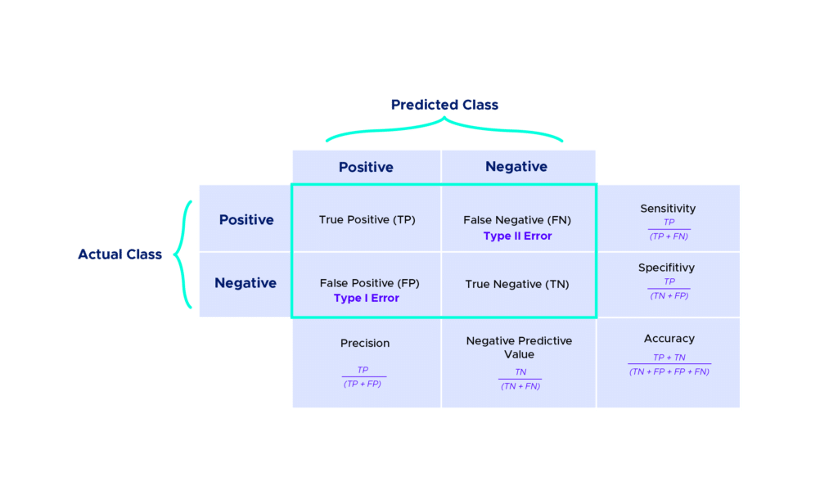
\includegraphics{img/cm.png}
\end{frame}

\begin{frame}{Bias/Variance Trade-off (Underfitting \& Overfitting)}
\protect\hypertarget{biasvariance-trade-off-underfitting-overfitting}{}
\includegraphics{img/Capture d’écran 2022-07-06 à 00.49.48.png}
\end{frame}

\begin{frame}{Bias/Variance Trade-off (Underfitting \& Overfitting)}
\protect\hypertarget{biasvariance-trade-off-underfitting-overfitting-1}{}
\includegraphics{img/Capture d’écran 2022-07-06 à 00.50.26.png}
\end{frame}



\end{document}
